\chapter{State of the Art}
\label{cha:state_of_the_art}

This chapter contains descriptions of the three most relevant papers for this thesis that are related to the topic
of monitoring in the context of microservices and cloud applications. In Section \ref{sec:cm_literature}
the three papers are sorted into the C\&M LITERATURE with a brief description of their content
and why they should be included in the C\&M LITERATURE. Section \ref{sec:uf+22}
contains a more detailed description of the paper that is most relevant to this thesis
and how it was used in this thesis.

\section{Analysis of and Contributions to the C\&M Literature}
\label{sec:cm_literature}

The C\&M LITERATURE is a list of publications that is maintained by the C\&M research group.
The publications contained in this list are relevant to the different areas of research of the group.
The list is split into five topics. Figure \ref{fig:categories_subcategories} shows an overview of these five categories and
sorts the three papers, described in this section, into these categories. The first topic is Engineering which contains publications
by the C\&M research group itself as well as publications that relate to the different phases
of the general software development process. The second topic is Analysis, Architecture, and Testing.
This topic contains publications that are relevant for modeling software and testing it.
The third topic, Authorization and Policies, focuses on access control for microservice-based applications.
The fourth topic, CI/CD and DevOps, contains publications related to the DevOps concept,
cloud-based software, and observability. Lastly, the fifth topic contains a mix of different publications
that were deemed relevant for the C\&M LITERATURE but do not fit into the other topics.

\begin{figure}[tb]
    \centering
    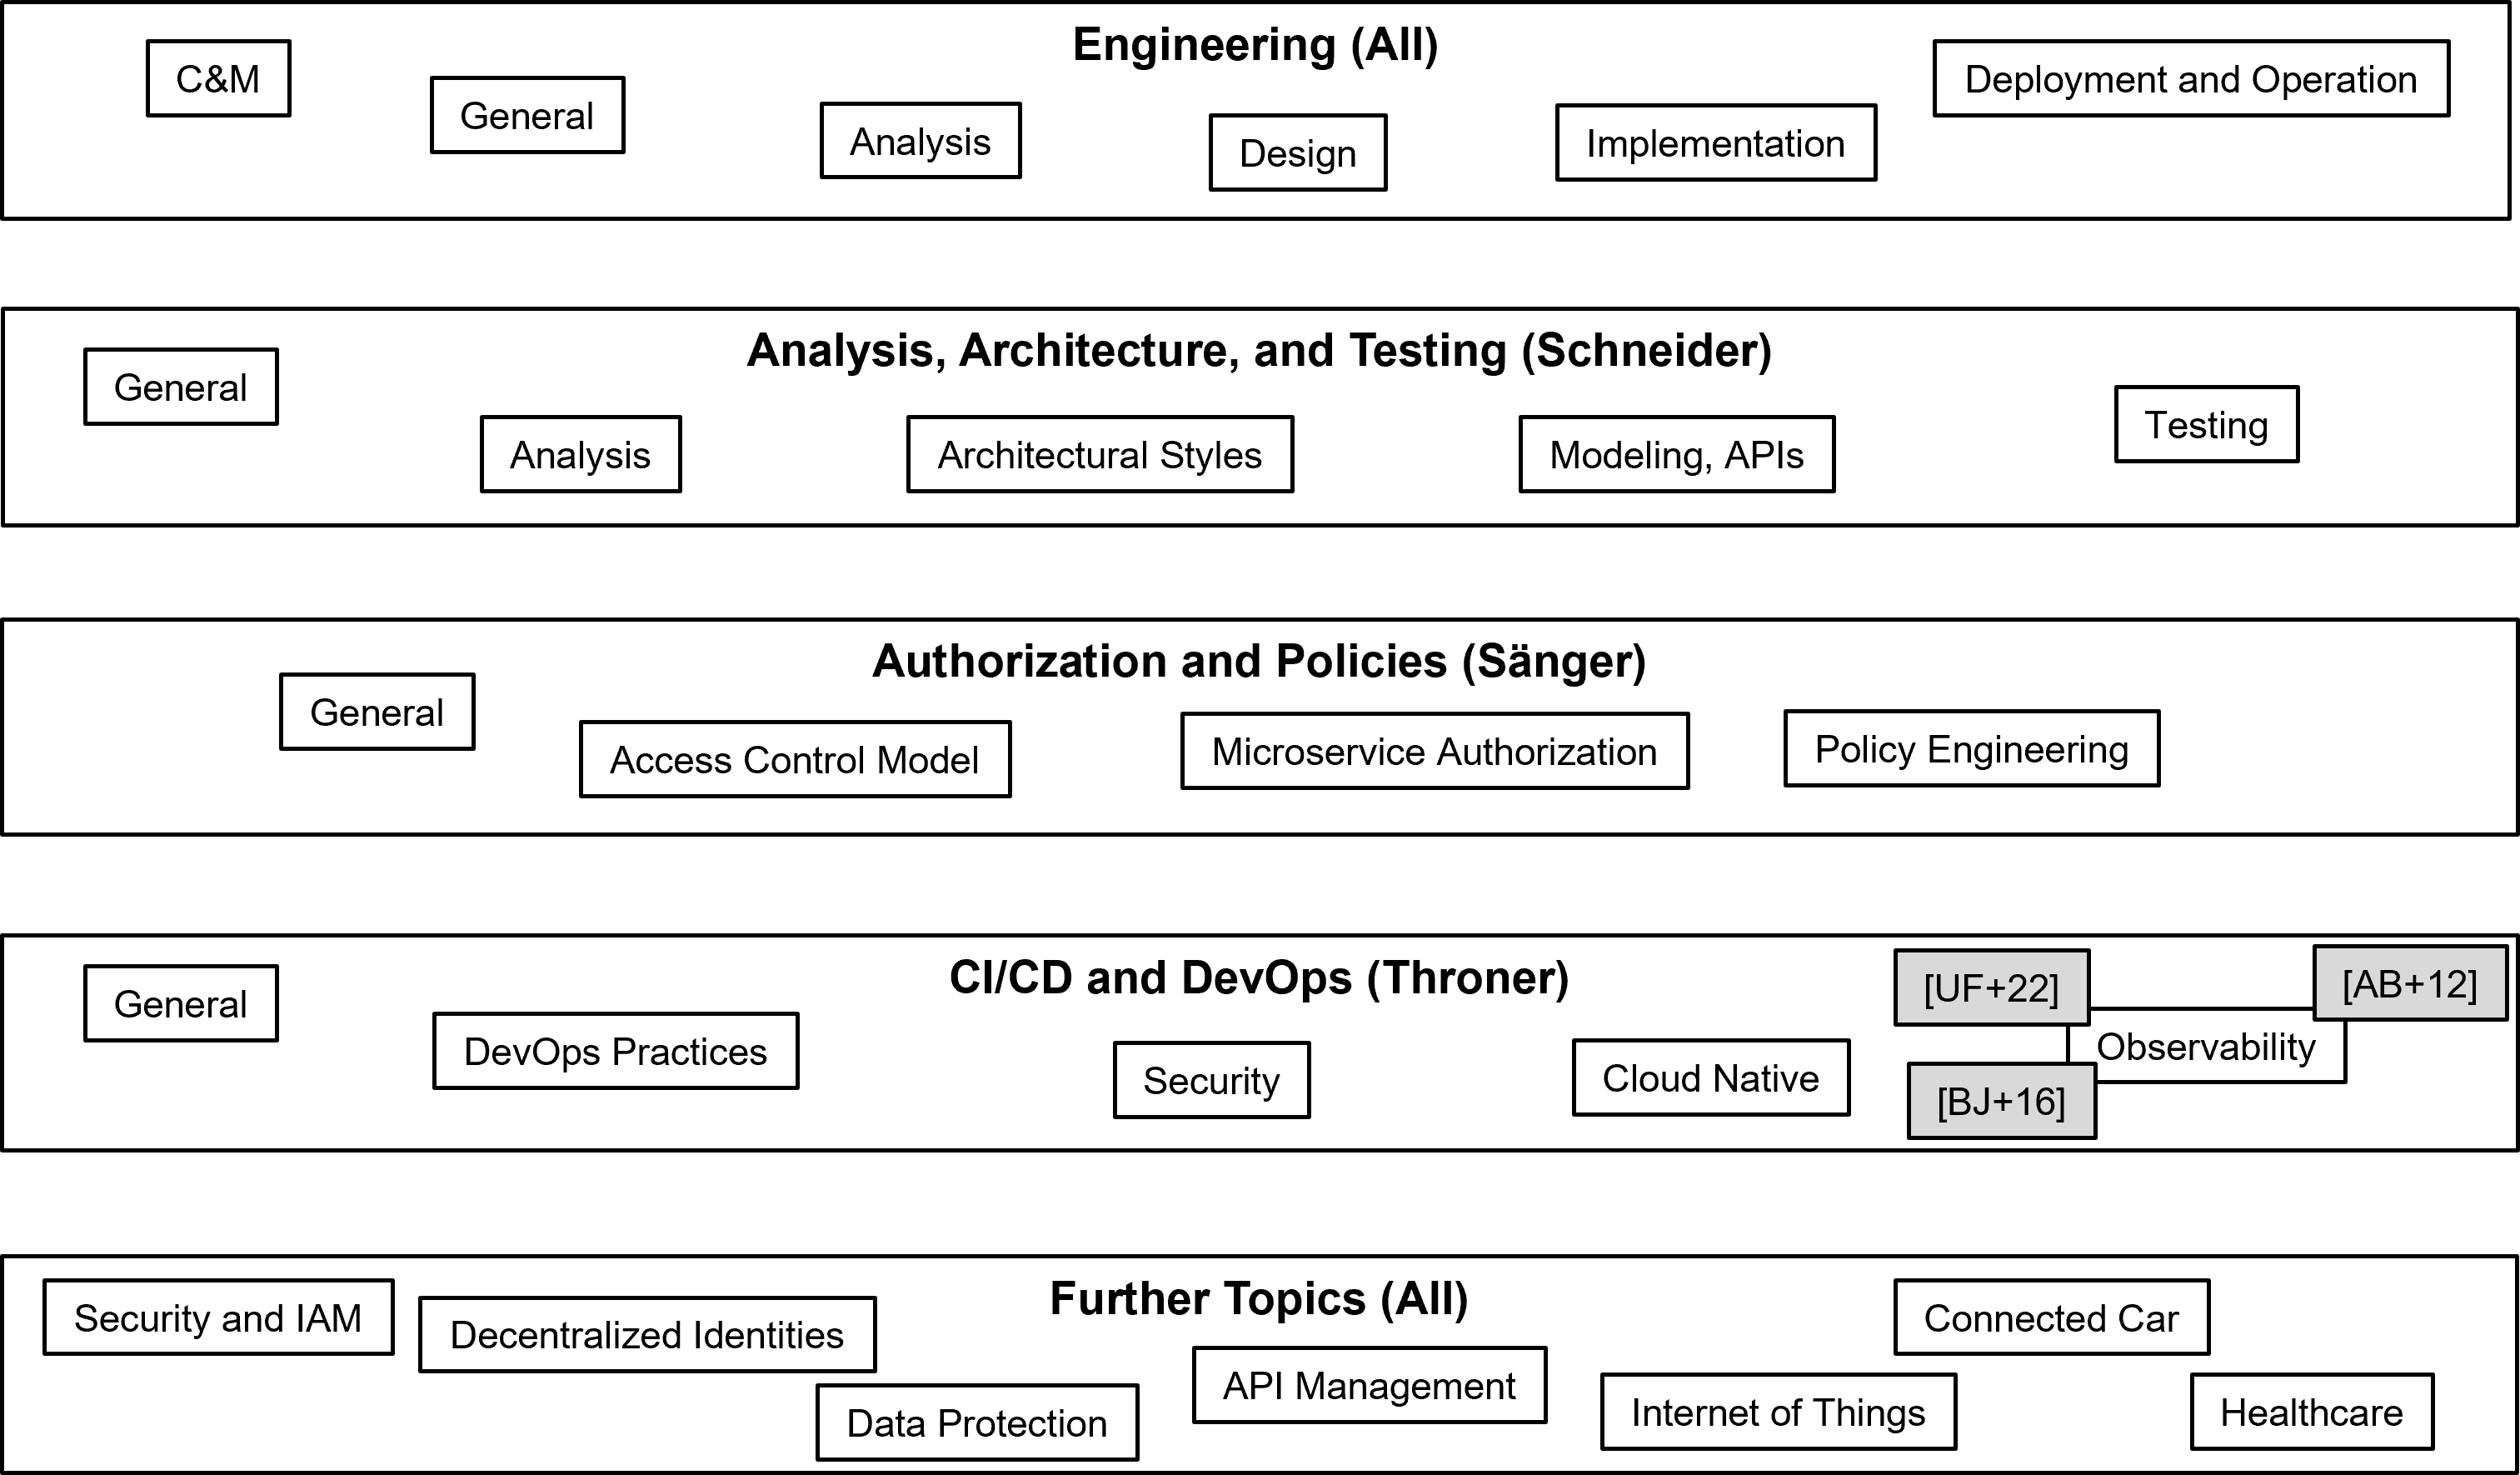
\includegraphics[width=\linewidth]{figures/literature.png}
    \caption{Categories and Subcategories}
    \label{fig:categories_subcategories}
\end{figure}

\subsection*{A Survey on Observability of Distributed Edge \& Container-Based Microservices \cite{UF+22}}

This paper provides a survey of state-of-the-art monitoring solutions.
The paper surveyed different monitoring solutions from academic papers as well as
commercial options. The monitoring solutions were analyzed regarding their scope,
their structure (multi-tenant and multi-layer), the instrumentation they provide (metrics, logs, and tracing),
and whether they are open-source solutions or not. The survey is summarized in a large table
which is followed by a description of each monitoring solution that was surveyed.
Additionally, the paper defines the data needed by an observability system, its basic functionalities,
and its key characteristics. For the context of C\&M, the paper provides a good overview of
both academic and commercial monitoring systems which can be used to investigate
different monitoring solutions in the future.

Status: CREATE (the publication should become a part of the C\&M LITERATURE  (09.09.2023))

\subsection*{Site Reliability Engineering \cite{BJ+16}}

This book by Beyer et al. \cite{BJ+16} discusses how Google develops reliable software
at some of the largest known scales. The authors of the book work in the Site Reliability Team
at Google. Site Reliability Engineering is the practice of using automated tooling
to increase the reliability of large-scale software systems.
The book is divided into five parts. The first part, introduction, introduces
the basic concepts needed by the rest of the book. In the second part, principles,
the book discusses seven principles on which the work of the Site Reliability Team
at Google is based. Part three, practices, goes into detail on the various tasks
of the Site Reliability Team which range from testing and monitoring to incident management.
Part four, management, explains the management aspects of running a Site Reliability Team.
Part five, conclusions, lists lessons learned from other industries and concludes the book.
For the context of C\&M, the book provides interesting insights into large-scale cloud software
systems which are mostly kept as close company secrets. 

Status: CREATE (the publication should become a part of the C\&M LITERATURE  (09.09.2023))

\subsection*{Cloud monitoring: Definitions, issues and future directions \cite{AB+12}}

This paper by Aceto et al. \cite{AB+12} discusses the motivation for monitoring cloud applications
as well as basic concepts and definitions of cloud monitoring. The paper starts by defining
eight tasks of cloud computing for which monitoring is required. This is followed by describing
cloud architecture as consisting of seven layers. Then eight properties are proposed that
a cloud monitoring system should possess. Finally, the paper reviews open issues and future
directions for the research into cloud monitoring. For the context of C\&M,
this paper provides some fundamental definitions for the area of monitoring cloud applications.

Status: CREATE (the publication should become a part of the C\&M LITERATURE  (09.09.2023))

\section{Usman et al.: A Survey on Observability of Distributed Edge \& Container-Based Microservices}
\label{sec:uf+22}

The paper A Survey on Observability of Distributed Edge \& Container-Based Microservices by Usman et al. \cite{UF+22}
was used by this thesis as an entry point into the topic of monitoring cloud-based software.
The paper discusses some of the fundamentals of monitoring like the three pillars of observability
and the four golden signals. Additionally, this paper defines the basic functionalities and key characteristics of an observability system.
While these definitions were not used as explicit goals for the development of the monitoring system in Chapter \ref{cha:first_solution},
they were used as guidelines during the development of the monitoring system and guided different decisions.

While the paper provides important fundamentals for monitoring and observability in general, the key goal of the paper
was a survey of modern observability solutions both from academia and the industry.
In total, the paper compared 43 different solutions based on their scope, whether they support multi-tenancy or multi-layer observability,
which pillars of observability are captured by the solutions and if they are open source or not.
This list was used as a basis for selecting the different components of the monitoring system developed in Chapter \ref{cha:first_solution}.
